\documentclass[pagesize=a4]{scrreprt}

\title{Implementing Gauss's Lemma in Lean}
\author{Aditya Agarwal}

\usepackage{amsmath}
\usepackage{amsthm,amssymb} 
\usepackage{listings}
\usepackage{graphicx} 
\usepackage[utf8x]{inputenc}

\newcommand{\R}{\mathbb{R}}
\newcommand{\N}{\mathbb{N}}
\newcommand{\Z}{\mathbb{Z}}
\newcommand{\Q}{\mathbb{Q}}
\newcommand{\C}{\mathbb{C}}
\newcommand{\F}{\mathbb{F}}

\newtheorem{theorem}{Theorem}
\newtheorem{definition}{Definition}
\newtheorem{lemma}{Lemma}

\begin{document}
\maketitle

\chapter{Background}

I attempted to implement a proof of Gauss's Lemma in Lean over the Australian summer of 2018-2019. This report provides the background on Lean and the Gauss Lemma, and details my (yet incomplete) proof.  

\section{Lean}

Lean is an Interactive theorem prover that implements mathematics using a form of dependent type theory known as the Calculus of Inductive Constructions. 

\subsection{Interactive Theorem Proving}

Interactive Theorem Provers are tools for writing proofs in formal mathematics that seek to abstract away the low level busy work. They work by having humans guide them by suggesting which ``tactic'' to use, and showing what they have inferred. For example 

For example, to prove that any reducible non-unit can be written as a product of two non-units, we may want to work with the definition of irreducibility. 

\smallskip

\begin{center}

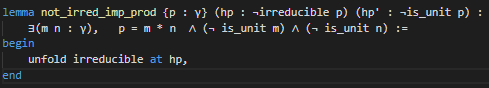
\includegraphics{tactic_example.png}\footnote{Forgive the code screenshots. Getting Unicode to work in \LaTeX turned out to be rather daunting. }

\end{center}
\smallskip

So we can tell the theorem prover to unfold the definition of irreducibility, at which point it will inform us on what the new state of the proof is. 

\smallskip
\begin{center}

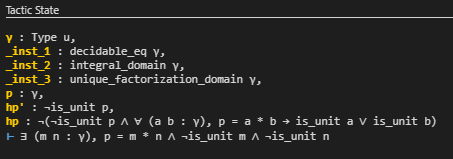
\includegraphics{tactic_state.png}

\end{center}
As we can see here, it has updated \texttt{hp} be $\neg$(definition of irreducibility). So by specifying which tactic to use, we may guide the theorem prover towards the proof. 

These tactics help the prover generate a proof, that is fed into a proof verifier, which then checks the correctness of the proof. 

In Lean, we may also interface with the proof verifier directly, in what is known as ``term mode''. 

For example, we show $0 + x = x$ by induction. Here $s$ is the successor operation, and $z$ is zero. 


\smallskip

\begin{center}

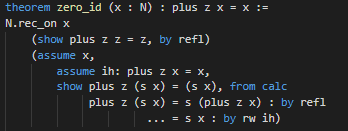
\includegraphics{term_example.png}

\end{center}

\subsection{Dependent Type Theory}

The Calculus of Constructions that Lean implements is a form of Dependent Type Theory, an alternative axiomatisation of mathematics. Rather than being constructed out of sets, each object has a fixed type, that type belongs to some universe $u$. 

For example, 

\begin{itemize}
    \item $n : \N$ $n$ belongs to the type of natural numbers. 
    \item $p \iff  p : Prop$ - $p \iff p$ is a proposition, which is also a type. 
\end{itemize}

This type may depend on a parameter such as 

\begin{itemize}
  \item $\text{list } \alpha$
  \item $\text{polynomial } \alpha$
\end{itemize}

We also have the notion of $\Pi$-types and $\Sigma$-types, which build new types out of other types. 

$\Pi$ types denote the notion of a dependent function type. A function whose return type may depend on the input parameter. E.g. the function $f(a) := x + a$ that takes an $a$ in any ring $\alpha$, returns $x + a$ in $\alpha[x]$

$$C :\Pi\ \alpha : \texttt{Type u}, \alpha \rightarrow \texttt{polynomial } \alpha $$

Similarly, $\Sigma$-types denote the cartesian product, where the type for the second element is allowed to depend on the first. 

i.e. $\Sigma\ \alpha\ \beta$ denotes the type $\alpha \times \beta$, where $\beta$ is allowed to depend on the type of $ \alpha$. 

\subsection{Mathlib}

Mathlib is the mathematical components library for Lean. 

It contains the beginnings of Algebra, Analysis, Topology, some elementary Number Theory. On the Algebra side, it contains basic definitions about Groups, Rings, Modules etc. And properties about Integral Domains, Euclidean Domains, Unique Factorisation Domains etc. 

I initially wanted to do some Algebraic Number Theory, but found Galois Theory was missing entirely. So I chose to implement the Gauss Lemma, the first step towards implementing Galois Theory.\footnote{My first plan was to work all the way to the Fundamental Theorem of Galois Theory, but that $grossly$ overestimated how fast I could implement proofs in Lean.} 

\section{Gauss's Lemma}

Before implementing it in Lean, we recall the statement and proof the Gauss Lemma. 

\begin{theorem}[Gauss's Lemma]
    Let $\alpha$ be a Unique Factorisation Domain. 

    Let $p$ be a polynomial with coefficients in $\alpha$. Then $p$ factors in $\alpha[X]$ if and only if it factors in $Frac(\alpha)[X]$.
\end{theorem}

Before we can prove Gauss's Lemma, we need to prove Gauss's Primitive Polynomial Lemma. 

\begin{definition}[Primitive Polynomial]

    Let $p$ be a polynomial in $\alpha[X]$. We say $p$ is primitive if the only constants in $ \alpha $ which divide $p$ are units. 

\end{definition}


\begin{lemma}[Gauss's Primitive Polynomial Lemma]
    Let $p$ and $q$ be primitive polynomials. Then $pq$ is a primitive polynomial.
\end{lemma}

\begin{proof}
    Assume for a contradiction that $pq$ is not primitive. 
    Then we have some $c \in \alpha$ such that $c$ is not a unit and $c \mid p$. 
   
    $\alpha$ is a UFD, so $c$ has some irreducible factor that divides $pq$. So WLOG, we may assume $c$ is irreducible, and hence prime.

    $\therefore \alpha/(c)$ is a domain.
    
    $\therefore \alpha/(c) [x]$ is a domain. 

    $c \mid pq$ so $pq$ vanishes in $\alpha/(c) [x]$. 

    As $\alpha/(c) [x]$ is an Integral Domain, $p$ vanishes or $q$ vanishes in $\alpha[X]$.

   $\therefore c \mid p$ or $c \mid q$. 
    
   $\therefore$ Either $p$ is not primitive or $q$ is not primitive. 

   Contradiction.
  \end{proof}

  Now we prove Gauss's Lemma. 

  \begin{proof}

    Let $p$ be an irreducible in $\alpha$. Any irreducible term must be primitive, so we know $p$ is primitive. 

    Suppose for a contradiction that $p$ is not irreducible in $Frac (\alpha)$. 

    Then $p = ab$, for some $a,b \in Frac (\alpha)[x]$. 

    We may multiply $a$ and $b$ by some $c_1,c_2 \alpha$ so that $c_1a,c_2b$ have $\alpha$ coefficients. $c_1c_2p = c_1ac_2b$. 
    We can factor $c_1a$ to some $c_1'a'$ and $c_2b$ to $c_2'b'$, so that $a'$ and $b'$ are primitive. 

    Hence $p = \frac{c_1'c_2'}{c_1c_2}a'b'$.

    Let $k =  \frac{c_1'c_2'}{c_1c_2}$

    We note that $k$ must be in $\alpha$, because otherwise 
if $k$ is not in $\alpha$, it's denominator (in reduced form) must divide each coefficient of $a'b'$. This is because $p =  ka'b'$ has $\alpha$ coefficients. 
  
    Hence $a'b'$ is not primitive. But by the primitive polynomial lemma, we know $a'b'$ is primitive. This is a contradiction. 

    But now we have produced a non-trivial factorisation for $p$ in $\alpha[X]$, namely $ka'b'$. This is a contradiction. 
    
    So it follows that if p is irreducible in  $\alpha[X]$ is irreducible in $Frac(\alpha[X])$


  \end{proof}


\chapter{Implementation} 

\chapter{Issues}

\end{document}